 \let\negmedspace\undefined
\let\negthickspace\undefined
\documentclass[journal]{IEEEtran}
\usepackage[a5paper, margin=10mm, onecolumn]{geometry}
\usepackage{lmodern} % Ensure lmodern is loaded for pdflatex
\usepackage{tfrupee} % Include tfrupee package

\setlength{\headheight}{1cm} % Set the height of the header box
\setlength{\headsep}{0mm}     % Set the distance between the header box and the top of the text

\usepackage{gvv-book}
\usepackage{gvv}
\usepackage{subfig}
\usepackage{cite}
\usepackage{amsmath,amssymb,amsfonts,amsthm}
\usepackage{algorithmic}
\usepackage{graphicx}
\usepackage{textcomp}
\usepackage{xcolor}
\usepackage{txfonts}
\usepackage{listings}
\usepackage{enumitem}
\usepackage{mathtools}
\usepackage{gensymb}
\usepackage{comment}
\usepackage[breaklinks=true]{hyperref}
\usepackage{tkz-euclide} 
\usepackage{listings}                                      
\def\inputGnumericTable{}                                 
\usepackage[latin1]{inputenc}                                
\usepackage{color}                                            
\usepackage{array}                                            
\usepackage{longtable}
\usepackage{multicol}
\usepackage{calc}                                             
\usepackage{multirow}                                         
\usepackage{hhline}                                           
\usepackage{ifthen}                                           
\usepackage{lscape}
\begin{document}

\bibliographystyle{IEEEtran}
\vspace{3cm}

\title{Scientific Calculator}
\author{EE24BTECH11052 - Rongali Charan}
% \maketitle
% \newpage
% \bigskip
{\let\newpage\relax\maketitle}

\renewcommand{\thefigure}{\theenumi}
\renewcommand{\thetable}{\theenumi}
\setlength{\intextsep}{10pt} % Space between text and floats


\numberwithin{equation}{enumi}
\numberwithin{figure}{enumi}
\renewcommand{\thetable}{\theenumi}
\tableofcontents
\newpage

\section{\textbf{Aim}}
Constructing the Scietific Calculator and using avr-gcc

    \section{ \textbf{Materials Required}}
\begin{itemize}
 \item  One 16X2 LCD display
    \item 5k$\Omega$ Potentiometer
    \item 2 X 180$\Omega$ resistors (for common anode current limiting)
    \item Bread Board
    \item Arduino UNO(atmega328p) and connecting cable
    \item Jumper wires for arduino and normal wires for seven segment displays
    \item Push Buttons(as many functions as needed)
\end{itemize}
\section{Hardware Setup}
The wiring process involves connecting the LCD display,Potentiometer to the Arduino pins.
\begin{figure}[H]
    \centering
    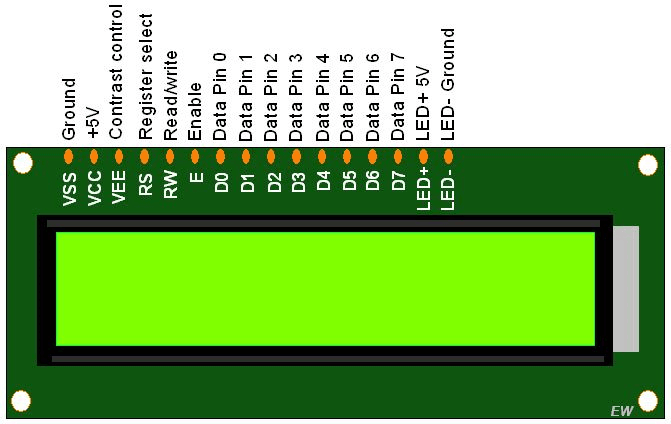
\includegraphics[width=0.6\linewidth]{Figs/LCD.png}
    \caption{LCD Display}
    \label{fig:enter-label}
\end{figure}



\subsection{LCD Connections}
\begin{center}
\begin{tabular}{|c|c|c|c|}
    \hline
    \textbf{LCD Pin} & \textbf{Function} & \textbf{Arduino Pin} & \textbf{Additional Components} \\
    \hline
    1 (VSS)  & Ground          & GND     & --- \\
    2 (VDD)  & Power Supply    & 5V      & --- \\
    3 (V0)   & Contrast Control &  180 $\Omega$ Resistor & Potentiometer (5k$\Omega$) \\
    4 (RS)   & Register Select  & D2      & --- \\
    5 (RW)   & Read/Write       & GND     & --- \\
    6 (E)    & Enable Signal    & D3      & --- \\
    7 (D0)   & Data Bit 0       & ---     & Not used \\
    8 (D1)   & Data Bit 1       & ---     & Not used \\
    9 (D2)   & Data Bit 2       & ---     & Not used \\
    10 (D3)  & Data Bit 3       & ---     & Not used \\
    11 (D4)  & Data Bit 4       & D4      & --- \\
    12 (D5)  & Data Bit 5       & D5      & --- \\
    13 (D6)  & Data Bit 6       & D6      & --- \\
    14 (D7)  & Data Bit 7       & D7      & --- \\
    15 (LED+) & Backlight Power  & 5V      & ---\\
    16 (LED-) & Backlight Ground & GND     & --- \\
    \hline
\end{tabular}
\end{center}

\subsection{Button Connections}

\begin{center}
\begin{tabular}{|c|c|c|}
    \hline
    \textbf{Button Index} & \textbf{Function} & \textbf{Arduino Pin} \\
    \hline
    0  & Button 0         & D8  \\
    1  & Button 1         & D9  \\
    2  & Button 2         & D10  \\
    3  & Button 3         & D11  \\
    4  & Button 4         & D12  \\
    5  & Button 5         & A0  \\
    6  & Button 6         & A1  \\
    7  & Button 7         & A2   \\
    8  & Button 8         & A3   \\
    9  & Button 9         & A4  \\
    Shift Button & Shift Mode       & A5    \\
    Extra Button & Extra Function   & D13   \\
    \hline
\end{tabular}
\end{center}

\section{Circuit Details}
\begin{itemize}
    \item The potentiometer (5k$\Omega$) is connected between the  VDD (5V)  and  GND  pins, with the wiper going to  V0 (LCD pin 3)  to control the contrast.
    \item The LCD's  backlight (LED+)  is powered by  5V  and  LED-  is connected to  GND .
\end{itemize}

\section{Common Issues}
\subsection*{Floating Pins and False Triggering}
\textbf{Problem:} When a button is not pressed, the pin might be in a floating state (neither HIGH nor LOW), causing false button presses or multiple triggers. \\
\textbf{Cause:} Without a resistor, the input pin may pick up noise or undefined signals, causing random fluctuations. \\
\textbf{Symptoms:}
\begin{itemize}
    \item Random and unexpected button presses.
    \item Inconsistent calculator behavior.
\end{itemize}
\textbf{Solution:}
\begin{itemize}
    \item Use external pull-down resistors (10k$\Omega$) or activate internal pull-up resistors to ensure stable pin states.
\end{itemize}

\subsection*{Button Debouncing Issues}
\textbf{Problem:} Mechanical bouncing during button presses generates multiple signals, resulting in repeated key registrations. \\
\textbf{Cause:} No debounce mechanism is applied, allowing multiple signals from a single press. \\
\textbf{Symptoms:}
\begin{itemize}
    \item Multiple digits displayed for a single press.
    \item Erratic or unexpected calculator operations.
\end{itemize}
\textbf{Solution:}
\begin{itemize}
    \item Implement a debouncing mechanism in software or use capacitors to filter out noise.
\end{itemize}

\subsection*{Excessive Power Consumption}
\textbf{Problem:} When buttons are pressed without resistors, a direct short may occur, causing excessive current draw. \\
\textbf{Cause:} Direct shorting without resistance protection. \\
\textbf{Symptoms:}
\begin{itemize}
    \item Potential damage to the Arduino board.
    \item Overheating or instability.
\end{itemize}
\textbf{Solution:}
\begin{itemize}
    \item Use current-limiting resistors (180-220 $\Omega$) to prevent high current flow.
    \item Enable internal pull-ups as a temporary solution.
\end{itemize}

\subsection*{Voltage Spikes and EMI Issues}
\textbf{Problem:} Button presses without resistors can generate voltage spikes and electromagnetic interference (EMI), disrupting the Arduino's stability. \\
\textbf{Cause:} Inductive effects and lack of resistance create transients. \\
\textbf{Symptoms:}
\begin{itemize}
    \item Random resets of the Arduino.
    \item Display glitches or freezing.
\end{itemize}
\textbf{Solution:}
\begin{itemize}
    \item Add small capacitors (0.1 $\mu$F) in parallel with the buttons to suppress noise.
    \item Use software filtering techniques to smooth out transient signals.
\end{itemize}

\subsection*{Incorrect Pin States and Code Logic Issues}
\textbf{Problem:} Without resistors, the default pin state may fluctuate randomly, causing incorrect button readings. \\
\textbf{Cause:} Floating pins lead to unstable logic detection. \\
\textbf{Symptoms:}
\begin{itemize}
    \item Inaccurate or unpredictable button presses.
    \item Incorrect calculations or display errors.
\end{itemize}
\textbf{Solution:}
\begin{itemize}
    \item Use internal pull-up resistors or add external resistors to prevent floating states.
\end{itemize}

\section*{Key Takeaway}
Even though resistors on buttons are not mandatory, using pull-down or pull-up resistors (either internal or external) ensures:
\begin{itemize}
    \item Stable and reliable input readings.
    \item Prevention of floating states and false triggering.
    \item Avoidance of unwanted behavior such as multiple or missed triggers.
\end{itemize}

\textbf{Recommendation:} Use internal pull-up resistors to avoid the need for external resistors while maintaining stable behavior.







\section{Code Implementation}
\section*{LCD Display Functions}
The calculator interfaces with an LCD to display results. The key functions include:
\begin{itemize}
    \item \texttt{lcd\_init()} - Initializes the LCD.
    \item \texttt{lcd\_cmd(command)} - Sends commands to the LCD.
    \item \texttt{lcd\_write(char data)} - Writes a character to the LCD.
    \item \texttt{lcd\_clear()} - Clears the screen.
    \item \texttt{lcd\_print(const char* str)} - Prints a string.
\end{itemize}

\section*{Mathematical Functions}

\subsection*{Square Root: Newton-Raphson Method}
The square root of a number \( x \) is computed using the iterative Newton-Raphson method:
\[
x_{n+1} = \frac{1}{2} \left( x_n + \frac{S}{x_n} \right)
\]
The implementation starts with an initial guess and iterates until convergence.

\begin{lstlisting}[language=C, caption=Square Root Function]
double my_sqrt(double S) {
    double x = S / 2.0;
    for (int i = 0; i < 10; i++) {
        x = 0.5 * (x + S / x);
    }
    return x;
}
\end{lstlisting}

\subsection*{Trigonometric Functions}
Trigonometric functions are computed using Taylor series approximations.

\subsubsection*{Sine Function}
The sine function is computed using:
\[
\sin(x) = x - \frac{x^3}{3!} + \frac{x^5}{5!} - \frac{x^7}{7!} + \dots
\]
\begin{lstlisting}[language=C, caption=Sine Function]
double my_sin(double x) {
    double term = x, sum = x;
    for (int n = 1; n < 10; n++) {
        term *= -x * x / ((2 * n) * (2 * n + 1));
        sum += term;
    }
    return sum;
}
\end{lstlisting}

\subsubsection*{Cosine Function}
Similarly, cosine is computed as:
\[
\cos(x) = 1 - \frac{x^2}{2!} + \frac{x^4}{4!} - \frac{x^6}{6!} + \dots
\]
\begin{lstlisting}[language=C, caption=Cosine Function]
double my_cos(double x) {
    double term = 1, sum = 1;
    for (int n = 1; n < 10; n++) {
        term *= -x * x / ((2 * n - 1) * (2 * n));
        sum += term;
    }
    return sum;
}
\end{lstlisting}

\subsubsection*{Tangent Function}
The tangent function is computed using:
\[
\tan(x) = \frac{\sin(x)}{\cos(x)}
\]
\begin{lstlisting}[language=C, caption=Tangent Function]
double my_tan(double x) {
    return my_sin(x) / my_cos(x);
}
\end{lstlisting}

\subsection*{Logarithm (Natural Log)}
The natural logarithm is computed using a series expansion for \( x > 0 \):
\[
\ln(1+x) = x - \frac{x^2}{2} + \frac{x^3}{3} - \frac{x^4}{4} + \dots
\]
\begin{lstlisting}[language=C, caption=Natural Log Function]
double my_ln(double x) {
    double sum = 0, term = (x - 1) / (x + 1);
    double num = term * term;
    for (int i = 1; i < 10; i += 2) {
        sum += term / i;
        term *= num;
    }
    return 2 * sum;
}
\end{lstlisting}

\subsection*{Exponential Function}
The exponential function \( e^x \) is computed using:
\[
e^x = 1 + x + \frac{x^2}{2!} + \frac{x^3}{3!} + \dots
\]
\begin{lstlisting}[language=C, caption=Exponential Function]
double my_exp(double x) {
    double sum = 1, term = 1;
    for (int n = 1; n < 10; n++) {
        term *= x / n;
        sum += term;
    }
    return sum;
}
\end{lstlisting}

\section*{Expression Evaluation}
The calculator evaluates arithmetic expressions using a recursive parser. The expression is tokenized, and the order of operations is handled correctly.

\begin{lstlisting}[language=C, caption=Expression Parsing]
double evaluate_expression(const char* expr) {
    // Tokenizes and evaluates the expression recursively
}
\end{lstlisting}

\section{Conclusion}
This document provides a detailed explanation of the scientific calculator's implementation on the AVR platform. The calculator is capable of evaluating mathematical expressions and computing various functions such as square roots, trigonometric functions, logarithms, and exponentials using custom algorithms. 

The mathematical functions were implemented using iterative methods (e.g., Newton-Raphson for square root) and series expansions (e.g., Taylor series for trigonometric and exponential functions) to achieve reasonable accuracy without relying on the standard C math library. 

Additionally, the LCD interface functions ensure clear and user-friendly display of results. The recursive expression evaluator enables the calculator to handle complex arithmetic expressions efficiently. 

Overall, this project demonstrates how fundamental mathematical operations and expression parsing can be efficiently implemented on resource-constrained embedded systems like AVR microcontrollers.

\begin{figure}[H]
    \centering
    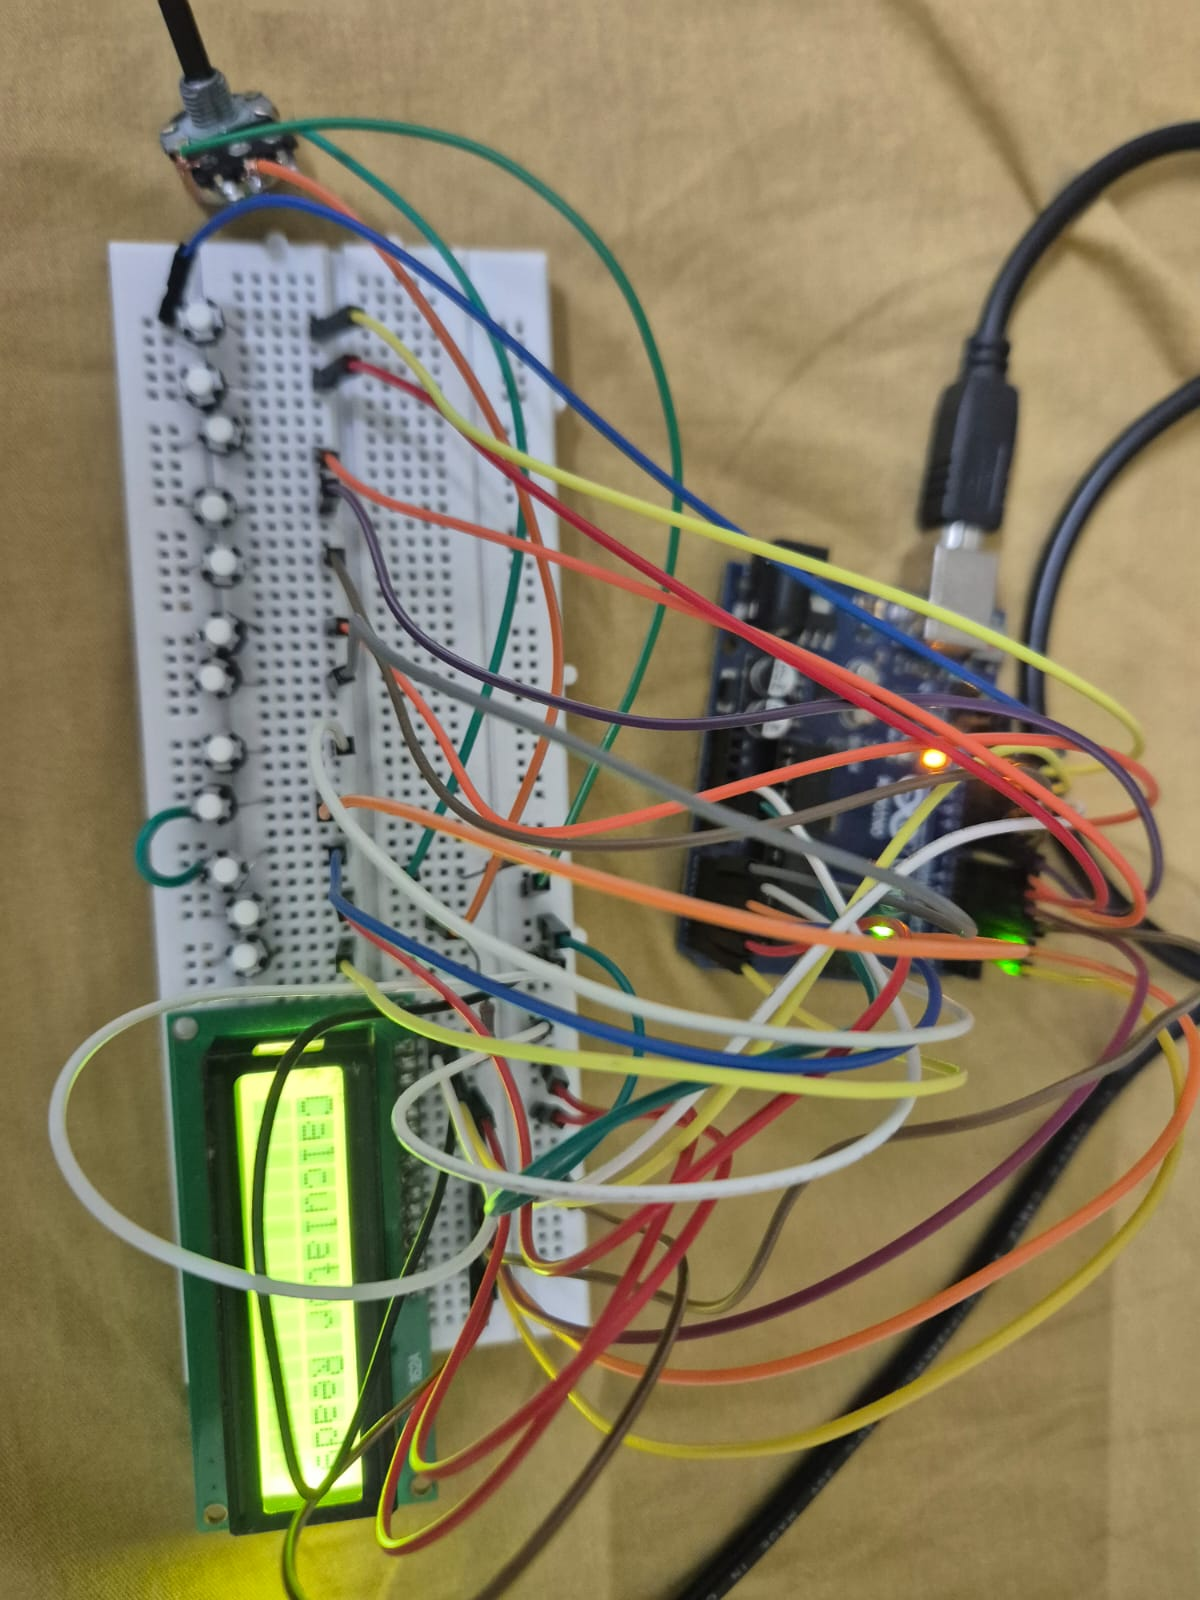
\includegraphics[width=0.7\linewidth]{Figs/calculator.png}
    \caption{Calculator}
    \label{fig:enter-label}
\end{figure}

\end{document}


\end{document}


%\end{document}